\documentclass[11pt,a4paper]{article}

\usepackage[utf8]{inputenc}
\usepackage[T1]{fontenc}
\usepackage{lmodern}
\usepackage{geometry}
\usepackage{microtype}
\usepackage{graphicx}
\usepackage{xcolor}
\usepackage{booktabs}
\usepackage{tabularx}
\usepackage{longtable}
\usepackage{array}
\usepackage{enumitem}
\usepackage{caption}
\usepackage{listings}
\usepackage[most]{tcolorbox}
\usepackage{tikz}
\usepackage{seqsplit}
\usepackage{hyperref}
\usepackage[nameinlink,noabbrev]{cleveref}

\usetikzlibrary{arrows.meta,positioning,shapes.geometric,fit,calc}

\geometry{top=2.45cm,bottom=2.55cm,left=2.65cm,right=2.65cm}
\linespread{1.03}
\raggedbottom
\setcounter{tocdepth}{1}
\setlength{\parskip}{0.35em}
\setlength{\parindent}{0pt}
\setlist[itemize]{leftmargin=1.15cm,itemsep=0.15em,topsep=0.25em}
\setlist[enumerate]{leftmargin=1.15cm,itemsep=0.15em,topsep=0.25em}
\captionsetup{font=small,labelfont=bf}

\definecolor{eurecomblue}{HTML}{009FE3}
\definecolor{deepblue}{HTML}{17324D}
\definecolor{softblue}{HTML}{EAF6FC}
\definecolor{softgray}{HTML}{F5F6F8}
\definecolor{rulegray}{HTML}{C8CDD3}
\definecolor{softamber}{HTML}{FFF7E6}
\definecolor{amberrule}{HTML}{D6A23A}
\definecolor{softred}{HTML}{FFF1F1}
\definecolor{redrule}{HTML}{B85C5C}
\definecolor{codebg}{HTML}{F7F7F7}

\hypersetup{
  colorlinks=true,
  linkcolor=deepblue,
  citecolor=deepblue,
  urlcolor=deepblue,
  pdftitle={Reproducibility Report for MeshAgent},
  pdfauthor={Jorge Echevarria de Uribarri}
}

\newcolumntype{Y}{>{\raggedright\arraybackslash}X}
\newcolumntype{L}[1]{>{\raggedright\arraybackslash}p{#1}}
\newcommand{\repo}{MeshAgent}
\newcommand{\dash}{--}
\newcommand{\commit}[1]{\texttt{#1}}
\newcommand{\commitlink}[2]{\href{https://github.com/Echeva26/MeshAgent/commit/#2}{\commit{#1}}}
\newcommand{\hash}[1]{\texttt{\scriptsize\seqsplit{#1}}}
\newcommand{\status}[1]{\textsc{#1}}

\lstdefinestyle{commandstyle}{
  basicstyle=\ttfamily\small,
  columns=fullflexible,
  keepspaces=true,
  breaklines=true,
  breakatwhitespace=true,
  showstringspaces=false,
  upquote=true
}

\newtcblisting{commandbox}[1][]{
  enhanced,
  breakable,
  listing only,
  listing options={style=commandstyle,language=bash},
  colback=codebg,
  colframe=rulegray,
  boxrule=0.45pt,
  arc=1mm,
  left=1.5mm,
  right=1.5mm,
  top=1mm,
  bottom=1mm,
  #1
}

\newtcolorbox{pendingbox}[1][]{
  enhanced,
  breakable,
  colback=softamber,
  colframe=amberrule,
  title=\textbf{Pending item},
  fonttitle=\small,
  coltitle=black,
  attach boxed title to top left={xshift=2mm,yshift=-2mm},
  boxed title style={colback=softamber,colframe=amberrule,boxrule=0.45pt,arc=1mm},
  boxrule=0.45pt,
  arc=1mm,
  left=2mm,
  right=2mm,
  top=3mm,
  bottom=2mm,
  #1
}

\newtcolorbox{missingbox}[1][]{
  enhanced,
  breakable,
  colback=softred,
  colframe=redrule,
  title=\textbf{Missing information},
  fonttitle=\small,
  coltitle=black,
  attach boxed title to top left={xshift=2mm,yshift=-2mm},
  boxed title style={colback=softred,colframe=redrule,boxrule=0.45pt,arc=1mm},
  boxrule=0.45pt,
  arc=1mm,
  left=2mm,
  right=2mm,
  top=3mm,
  bottom=2mm,
  #1
}

\newtcolorbox{evidencebox}[1][]{
  enhanced,
  breakable,
  colback=softblue,
  colframe=eurecomblue,
  title=\textbf{Evidence note},
  fonttitle=\small,
  coltitle=black,
  attach boxed title to top left={xshift=2mm,yshift=-2mm},
  boxed title style={colback=softblue,colframe=eurecomblue,boxrule=0.45pt,arc=1mm},
  boxrule=0.45pt,
  arc=1mm,
  left=2mm,
  right=2mm,
  top=3mm,
  bottom=2mm,
  #1
}

\begin{document}

\begin{titlepage}
  \centering
  \vspace*{1.0cm}
  \IfFileExists{figures/eurecom-logo-horizontal.png}{
    
\includegraphics[width=0.36\textwidth]{figures/eurecom-logo-horizontal.png}
  }{
    \fbox{\parbox{0.62\textwidth}{\centering Insert official EURECOM logo here}}
  }

  \vspace{2.0cm}
  {\Huge\bfseries Reproducibility Report for MeshAgent\par}
  \vspace{0.55cm}
  {\Large Analysis of the Implemented Work and Reproducibility Assessment\par}

  \vspace{2.4cm}
  {\Large Jorge Echevarria de Uribarri\par}
  \vspace{0.35cm}
  {\large EURECOM\par}

  \vfill
  {\large 5 June 2026\par}
  \vspace{0.4cm}
  {\footnotesize Logo source: EURECOM newsroom \cite{eurecomnewsroom}.}
\end{titlepage}

\pagenumbering{roman}
\tableofcontents
\newpage
\pagenumbering{arabic}

\begin{abstract}
This report evaluates the reproducibility of the current \repo{} repository as a technical artifact and as an empirical basis for LLM-assisted network-graph analysis. The repository has been migrated from an Azure-dependent implementation to a local, self-hostable stack based on vLLM, \texttt{sentence-transformers}, and Qdrant. That migration makes the system more inspectable and substantially easier to run than the upstream baseline, while preserving the original agentic workflow of retrieval, LLM code generation, execution, verification, and golden-answer comparison.

Following the reproducibility framework used in the provided NetLLM thesis \cite{rissanen2026netllm} and the ACM artifact criteria \cite{acm2020badging}, the report concludes that \repo{} is \emph{partially reproducible}. The code, graph data, prompt templates, RAG sources, persisted Qdrant collections, smoke-test scripts, and result logs are available. However, the exact model-serving environment is not fully specified, most dependencies are not pinned, vLLM is installed outside the repository dependency file, and the comparative model evaluation has not yet been executed. Consequently, the implementation is technically credible, but its empirical reproducibility remains incomplete.
\end{abstract}

\section{Introduction}

LLM-based systems complicate the ordinary meaning of a reproducible software artifact. Their behavior is shaped not only by source code and data, but also by model checkpoints, inference backends, prompt templates, vector indexes, hardware, and package versions. A small change in any of these layers can alter the generated output, especially when the LLM is part of the runtime system rather than merely a tool used during development.

The provided thesis on NetLLM frames this problem in the context of network research, where reproducing results requires attention to code availability, model availability, hardware constraints, dependency versions, seeds, and evaluation scripts \cite{rissanen2026netllm,wu2024netllm}. \repo{} belongs to the same broad family of systems: it uses an LLM to generate executable Python code for network and graph-analysis tasks, combines that generation with retrieval over constraints and tools, and evaluates outputs against verifiers and golden answers when possible.

The purpose of this report is therefore twofold. First, it documents the engineering work implemented in the repository, especially the migration away from cloud-specific Azure services toward a local stack. Second, it assesses how far the resulting artifact can support reproduction by an external evaluator. The answer is deliberately cautious: the repository is much more reproducible than the upstream baseline, but it is not yet a complete reproducibility package.

\section{Methodological Framework}

\subsection{Terminology}

This report follows the distinction used in the thesis and in the ACM artifact-review criteria \cite{rissanen2026netllm,acm2020badging}. \emph{Reproduction} refers to obtaining the same results using the same artifacts and experimental setup. \emph{Replication} refers to obtaining consistent results with a different or independently recreated setup. In this report, most claims concern reproduction of the current repository state. Claims about replication are limited, because the planned cross-model comparison has not yet been performed.

LLM-based artifacts present specific risks: dependency drift, unavailable model checkpoints, hidden prompts, non-deterministic inference, undocumented hardware requirements, unpinned vector-store state, and incomplete evaluation scripts. These risks are not abstract in \repo{}. They appear concretely in the need to start an external vLLM server, resolve Hugging Face-hosted models, rebuild or trust Qdrant collections, and interpret small result logs that are not statistically controlled benchmarks.

\subsection{Method of Assessment}

The assessment was produced through a repository audit rather than by relying on the repository documentation alone. The following evidence was inspected:

\begin{itemize}
  \item git history comparing \texttt{upstream/main} with the current \texttt{main} branch;
  \item README files, environment examples, dependency files, and benchmark documentation;
  \item the shared \texttt{common/} modules for configuration, LLM access, embeddings, vector search, RAG indexing, and graph compatibility;
  \item the three application entrypoints and helper modules;
  \item graph data, RAG JSON files, golden-answer files, persisted Qdrant metadata, and included result logs;
  \item smoke-test outcomes for embeddings, retrieval, and vLLM connectivity;
  \item the provided thesis PDF as the methodological reference.
\end{itemize}

\begin{evidencebox}
The current local branch is \texttt{main} at \commitlink{84218ab}{84218abadccb2a5f855f5bef4dcbe07b53af996a}. The upstream baseline used for comparison is \commit{0fb45c7}. Full hashes are listed in \cref{app:commits}; the narrative uses short hashes for readability.
\end{evidencebox}

\section{Baseline Repository State}

\subsection{Reconstructing the Baseline}

The baseline state can be reconstructed from git history rather than inferred from file names alone. The upstream branch points to \commit{0fb45c7}, after an initial import and cleanup. The current branch diverges after that point, with later commits adding the local execution stack, Qdrant configuration, smoke tests, result logs, and benchmark wrapper.

The upstream repository implemented an agentic graph-analysis workflow across three application directories: \texttt{app-malt}, \texttt{app-CRG}, and \texttt{app-traffic-analysis}. The workflow already had the essential MeshAgent structure: retrieve task constraints and tools, ask an LLM to produce a plan, generate Python code for a \texttt{process\_graph} function, execute that code on a graph, run verifier checks, self-debug failures, and compare outputs against golden answers when available.

\subsection{Baseline Dependencies and Reproducibility Limits}

The baseline was difficult to reproduce because its infrastructure depended on externally configured cloud services. The root README listed notebook-style package installation commands rather than a project-level dependency file. It also required Azure Search, Azure OpenAI or Google VertexAI configuration, and Jupyter notebooks for RAG index creation. The upstream \texttt{app-malt/ai\_models\_cot.py} used Azure GPT deployments such as \texttt{gpt-4-32k}; helper code imported Azure Search clients and vector-search classes.

This baseline was not unusable, but it was not self-contained. An evaluator needed credentials, service endpoints, model deployment names, Azure index names, and notebook execution steps. In the terminology of the ACM criteria, the artifacts were available but not straightforwardly exercisable \cite{acm2020badging}. The problem resembles the NetLLM reproduction issues discussed in the thesis: code availability alone does not guarantee reproduction if the environment, dependencies, and models are underspecified \cite{rissanen2026netllm}.

\section{Implemented Changes}

\subsection{Migration Logic}

The current implementation follows a coherent engineering strategy. It replaces credential-dependent cloud services with local components while leaving the original agentic control flow mostly intact. Instead of rewriting the graph-analysis pipeline, the implementation changes the provider layer underneath it.

The resulting stack has three local components: vLLM provides chat inference, Sentence-Transformers computes embeddings, and Qdrant stores and searches RAG constraints and tools. Configuration moves into \path{.env.example} and \path{common/config.py}. Retrieval moves into \path{common/vector_store.py}, while index construction moves from Azure notebooks into \path{scripts/build_qdrant_indexes.py}. \Cref{fig:architecture} summarizes the architectural change.

\begin{figure}[htbp]
  \centering
  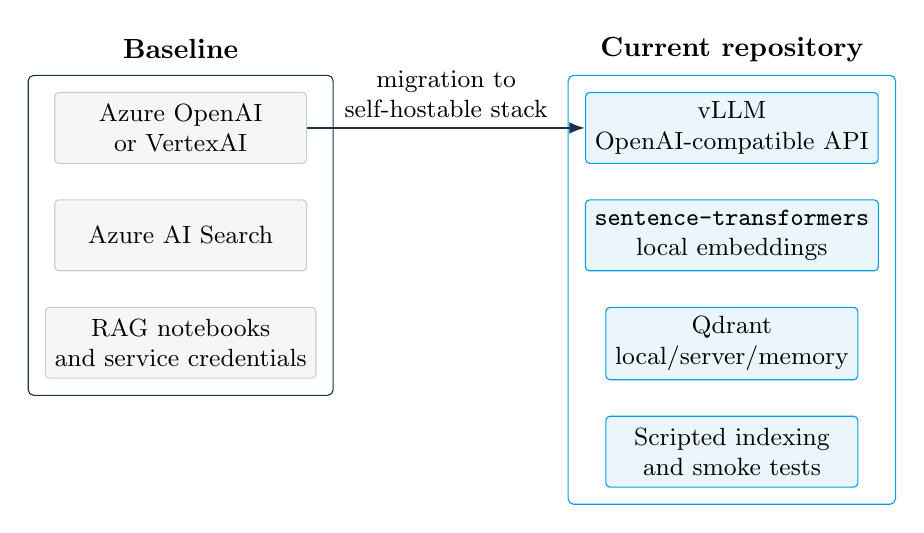
\begin{tikzpicture}[
    font=\small,
    box/.style={draw=rulegray,rounded corners=1.5pt,fill=softgray,align=center,minimum width=3.2cm,minimum height=0.9cm},
    cloud/.style={draw=eurecomblue,rounded corners=1.5pt,fill=softblue,align=center,minimum width=3.2cm,minimum height=0.9cm},
    arrow/.style={-{Latex[length=2mm]},thick,draw=deepblue}
  ]
    \node[font=\bfseries] (btitle) at (0,2.2) {Baseline};
    \node[box] (b1) at (0,1.2) {Azure OpenAI\\or VertexAI};
    \node[box,below=0.45cm of b1] (b2) {Azure AI Search};
    \node[box,below=0.45cm of b2] (b3) {RAG notebooks\\and service credentials};

    \node[font=\bfseries] (ctitle) at (7.0,2.2) {Current repository};
    \node[cloud] (c1) at (7.0,1.2) {vLLM\\OpenAI-compatible API};
    \node[cloud,below=0.45cm of c1] (c2) {\texttt{sentence-transformers}\\local embeddings};
    \node[cloud,below=0.45cm of c2] (c3) {Qdrant\\local/server/memory};
    \node[cloud,below=0.45cm of c3] (c4) {Scripted indexing\\and smoke tests};

    \node[draw=deepblue,rounded corners=2pt,fit=(b1)(b2)(b3),inner sep=6pt] {};
    \node[draw=eurecomblue,rounded corners=2pt,fit=(c1)(c2)(c3)(c4),inner sep=6pt] {};
    \draw[arrow] (b1.east) -- node[above,align=center]{migration to\\self-hostable stack} (c1.west);
  \end{tikzpicture}
  \caption{Conceptual architecture change from the upstream cloud-dependent baseline to the current local/self-hostable implementation.}
  \label{fig:architecture}
\end{figure}

\subsection{Commit Summary}

\begin{table}[htbp]
  \centering
  \caption{Concise implementation history.}
  \label{tab:commits}
  \begin{tabularx}{\textwidth}{L{2.3cm}L{4.2cm}Y}
    \toprule
    Short commit & Main change & Reproducibility impact \\
    \midrule
    \commitlink{7b099a2}{7b099a2d10eb212ba4a7b338a9d7cd99662865dd} & Local vLLM/Qdrant migration & Removes the hard dependency on Azure services and introduces shared local providers. \\
    \commitlink{9283e88}{9283e886a795f218daa8978394906590b513f5c3} & Flexible Qdrant modes & Allows embedded local storage, server mode, or memory mode. \\
    \commitlink{993f3d6}{993f3d6271c5307249702f53eb53256c7b719bcb} & Log-directory creation & Avoids failures caused by missing output directories. \\
    \commitlink{670e5c8}{670e5c847a128310ef66fba59a24f59c30546cce} & NetworkX compatibility & Handles node-link JSON differences between \texttt{links} and \texttt{edges}. \\
    \commitlink{9a80e9b}{9a80e9b7c9c208b06cc9776bc243d3fa755b5dcd} / \commitlink{db3b005}{db3b005e72b4ca60664b37b6c8825297ac7b72a4} & Missing-golden-answer handling & Allows inference-only or skipped runs instead of aborting the whole evaluation. \\
    \commitlink{6241057}{6241057e0f5fd38f9664ac6c8cf47cf459ed0d84} & Result and Qdrant artifacts & Provides inspectable logs and persisted local vector collections. \\
    \commitlink{84218ab}{84218abadccb2a5f855f5bef4dcbe07b53af996a} & Benchmark-result ignore rule & Keeps generated benchmark outputs out of normal repository churn. \\
    \bottomrule
  \end{tabularx}
\end{table}

The table deliberately compresses the commit history. The more important point is the migration path: the repository now has a provider layer that can be inspected and tested independently of the application prompts. This separation is the strongest engineering contribution from a reproducibility standpoint.

\section{Current Architecture and Toolchain}

\subsection{Execution Flow}

The current pipeline remains an LLM-driven code-generation system. Graph data are loaded from checked-in files, RAG retrieval selects relevant constraints and tools, prompt templates ask the LLM for a three-step plan and step-specific code, and the generated \texttt{process\_graph} function is executed. Verifier checks and self-debugging loops attempt to catch structural or execution failures before the final answer is compared with a golden answer.

\begin{figure}[htbp]
  \centering
  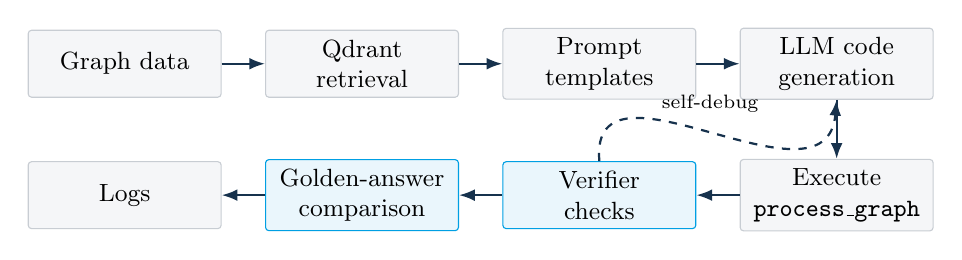
\begin{tikzpicture}[
    font=\small,
    flowstep/.style={draw=rulegray,rounded corners=1.2pt,fill=softgray,align=center,minimum width=2.45cm,minimum height=0.85cm},
    check/.style={draw=eurecomblue,rounded corners=1.2pt,fill=softblue,align=center,minimum width=2.45cm,minimum height=0.85cm},
    arrow/.style={-{Latex[length=2mm]},thick,draw=deepblue}
  ]
    \node[flowstep] (g) {Graph data};
    \node[flowstep,right=0.55cm of g] (r) {Qdrant\\retrieval};
    \node[flowstep,right=0.55cm of r] (p) {Prompt\\templates};
    \node[flowstep,right=0.55cm of p] (c) {LLM code\\generation};
    \node[flowstep,below=0.75cm of c] (x) {Execute\\\texttt{process\_graph}};
    \node[check,left=0.55cm of x] (v) {Verifier\\checks};
    \node[check,left=0.55cm of v] (a) {Golden-answer\\comparison};
    \node[flowstep,left=0.55cm of a] (l) {Logs};

    \draw[arrow] (g) -- (r);
    \draw[arrow] (r) -- (p);
    \draw[arrow] (p) -- (c);
    \draw[arrow] (c) -- (x);
    \draw[arrow] (x) -- (v);
    \draw[arrow] (v) -- (a);
    \draw[arrow] (a) -- (l);
    \draw[arrow,dashed] (v.north) to[out=95,in=-95,looseness=1.25]
      node[midway,above,font=\scriptsize,yshift=1mm]{self-debug} (c.south);
  \end{tikzpicture}
  \caption{Simplified \repo{} execution flow. The dashed arrow represents the self-debugging loop triggered by execution or verifier errors.}
  \label{fig:flow}
\end{figure}

\subsection{Toolchain}

The toolchain is now more transparent than in the upstream repository, but it remains a layered system. vLLM and the selected model define generation behavior \cite{kwon2023vllm,vllmdocs}; Sentence-Transformers and Qdrant define retrieval behavior \cite{reimers2019sentencebert,qdrantdocs}; NetworkX and app-specific helpers define graph semantics; and the evaluation scripts define what is counted as a pass or failure. \Cref{tab:tools} summarizes the most relevant components.

\begin{table}[htbp]
  \centering
  \caption{Main technical components and their reproducibility role.}
  \label{tab:tools}
  \begin{tabularx}{\textwidth}{L{3.0cm}Y Y}
    \toprule
    Component & Role & Reproducibility significance \\
    \midrule
    vLLM & Serves an OpenAI-compatible chat endpoint. & Makes local serving possible, but exact vLLM version, model revision, quantization, and hardware must be recorded. \\
    Qdrant & Stores and searches embedded constraints and tools. & Provides local vector-store state; rebuilds depend on embedding model and package versions. \\
    Sentence-\\Transformers & Computes local embeddings. & Removes Azure embedding dependence; still depends on a Hugging Face-hosted model unless cached or pinned. \\
    LangChain / OpenAI client & Provides chat and prompt interfaces. & Preserves existing chain structure; API behavior can drift across versions. \\
    NetworkX & Represents graph inputs and generated graph outputs. & Requires compatibility handling for node-link JSON formats. \\
    Benchmark wrapper & Runs smoke tests and app entrypoints across model endpoints. & Enables the pending cross-model evaluation, but no final benchmark output is present. \\
    \bottomrule
  \end{tabularx}
\end{table}

This stack is appropriate for a reproducibility-oriented migration because it moves the system toward inspectable local services. At the same time, it does not by itself guarantee reproducibility. The model-serving command, model revision, embedding revision, and package versions remain part of the experimental artifact and should be recorded with every final run.

\section{Experimental Setup and Available Evidence}

\subsection{Repository and Environment}

The inspected repository is \url{https://github.com/Echeva26/MeshAgent.git} \cite{meshagent2026repo}. The current branch is \texttt{main}; the baseline comparison uses \texttt{upstream/main}. During the audit, the local virtual environment used Python 3.14.2 on macOS arm64. This local environment is not necessarily the environment used to produce the included result logs.

\begin{missingbox}
The exact hardware, GPU model, vLLM version, CUDA version, PyTorch CUDA build, model revision, quantization mode, and model-serving command used for the included result logs are not recorded in the repository.
\end{missingbox}

\subsection{Data and Index Evidence}

The graph datasets are checked into the repository. Loading them from the required app directories produced the sizes shown in \cref{tab:datasets}. The need to run from app directories is not a cosmetic detail: the helpers use relative paths.

\begin{table}[htbp]
  \centering
  \caption{Checked-in graph datasets.}
  \label{tab:datasets}
  \begin{tabularx}{\textwidth}{L{3.0cm}rrY}
    \toprule
    App & Nodes & Edges & Source \\
    \midrule
    MALT & 5,493 & 6,424 & \path{app-malt/data/malt-example-final.textproto.txt} \\
    CRG & 200 & 1,034 & \path{app-CRG/data/resources.json} \\
    Traffic Analysis & 100 & 32 & \path{app-traffic-analysis/data/test_graph.json} \\
    \bottomrule
  \end{tabularx}
\end{table}

The RAG sources are also versioned: MALT has 15 constraints and 4 tools, CRG has 15 constraints and 2 tools, and Traffic Analysis has 10 constraints and 5 tools. The persisted Qdrant metadata contains matching collection counts, all using 384-dimensional cosine vectors, which is consistent with the default \texttt{all-MiniLM-L6-v2} embedding model.

\subsection{Smoke Tests}

The embedding and retrieval checks provide evidence that part of the local stack is functional. The embedding test initially required access to Hugging Face in order to resolve the configured model; after that access was available, it returned 384-dimensional vectors. The retrieval test against \texttt{app-malt} returned Qdrant constraint and tool matches. The vLLM test failed with connection refused, indicating that no OpenAI-compatible model server was listening at the configured endpoint during the audit.

These outcomes should be read carefully. They show that the local embedding and retrieval layers can run, not that the full application is currently reproducible end to end. Full execution still requires a separately installed and running vLLM server.

\section{Reproducibility Assessment}

\subsection{Logged Results}

The repository includes result logs for all three applications. They demonstrate that the pipeline has previously been run through code generation, execution, verification, and output comparison. They do not constitute a statistically controlled benchmark.

\begin{table}[htbp]
  \centering
  \caption{Summary of included result logs.}
  \label{tab:results}
  \begin{tabular}{lrrrr}
    \toprule
    App & Evaluated & Passed & Failed & Skipped \\
    \midrule
    MALT & 3 & 1 & 2 & 1 \\
    CRG & 0 & 0 & 0 & 3 \\
    Traffic Analysis & 6 & 3 & 3 & 1 \\
    \midrule
    Total & 9 & 4 & 5 & 5 \\
    \bottomrule
  \end{tabular}
\end{table}

Among prompts with golden answers, the included logs show a pass rate of \(4/9 = 44.4\%\). This number is useful only as a descriptive summary of the available logs. It is not a stable estimate of model performance because the sample is small, run metadata are incomplete, and some failures may reflect strict golden-answer matching rather than an unequivocally wrong answer. Conversely, verifier success alone does not prove semantic correctness: several logged failures passed structural checks but missed the intended aggregation or grouping.

The skipped cases are also informative. They show that the current code can avoid aborting when an exact golden-answer key is missing, but they also show that some active prompts are not aligned with the available evaluation set. For academic evaluation, the prompt list, golden-answer file, and result summary should be synchronized before the final run.

\subsection{Artifact Assessment}

\begin{table}[htbp]
  \centering
  \caption{Reproducibility assessment summary.}
  \label{tab:assessment}
  \begin{tabularx}{\textwidth}{L{3.8cm}L{2.1cm}Y}
    \toprule
    Criterion & Status & Rationale \\
    \midrule
    Artifacts available & \status{Yes} & Source code, graph data, prompts, RAG inputs, persisted Qdrant storage, and logs are present. \\
    Artifacts functional & \status{Partial} & Embedding and retrieval smoke tests passed; vLLM connectivity failed because no server was running. \\
    Environment reproducibility & \status{Partial} & Configuration is documented, but no lockfile, Dockerfile, Python version constraint, or vLLM version is provided. \\
    Dependency reproducibility & \status{Partial} & A \texttt{requirements.txt} exists, but most dependencies are unpinned and vLLM is installed separately. \\
    Model reproducibility & \status{Partial} & Model names are specified, but exact revisions, serving settings, and quantization are not recorded. \\
    Data and vector-store reproducibility & \status{Partial} & Data and Qdrant collections are present; regenerated embeddings may differ if model or package versions drift. \\
    Results reproducible & \status{Partial} & Logs demonstrate prior execution, but a full rerun requires the missing serving environment. \\
    Results replicable & \status{Pending} & The comparative model experiment has not yet been executed. \\
    \bottomrule
  \end{tabularx}
\end{table}

The overall assessment is therefore \textbf{partially reproducible}. The repository is no longer merely a cloud-dependent research prototype, but it still lacks the environmental precision required for independent reproduction of the included results from scratch.

\section{Pending Comparative Model Evaluation}

\begin{pendingbox}
The final comparative evaluation across open-source model backends has not been executed. This section records the planned experiment and the evidence required to complete it. Leaving the results pending is methodologically necessary: reporting synthetic or assumed benchmark values would misrepresent the current repository evidence.
\end{pendingbox}

The benchmark wrapper in \path{scripts/benchmark_opensource_models.py} is designed to run the existing smoke tests and application entrypoints across several OpenAI-compatible model endpoints. The example matrix lists Qwen2.5-Coder, DeepSeek-Coder, and StarCoder2 endpoints. Once the servers are running, the wrapper should collect return codes, durations, query counts, accuracy values, pass/fail counts, skipped counts, and captured stdout/stderr.

\begin{table}[htbp]
  \centering
  \caption{Planned comparative model results table.}
  \label{tab:pending-models}
  \begin{tabularx}{\textwidth}{YccccY}
    \toprule
    Model & Tests run & Successes & Mean accuracy & Duration & Notes \\
    \midrule
    Qwen2.5-Coder-14B-Instruct & Pending & Pending & Pending & Pending & Awaiting benchmark execution. \\
    DeepSeek-Coder-6.7B-Instruct & Pending & Pending & Pending & Pending & Awaiting benchmark execution. \\
    StarCoder2-15B-Instruct & Pending & Pending & Pending & Pending & Awaiting benchmark execution. \\
    \bottomrule
  \end{tabularx}
\end{table}

For the final submission, the benchmark output should also record GPU model, VRAM, vLLM version, CUDA version, PyTorch version, model revision, quantization mode, maximum context length, and exact server command for each model. Without that metadata, cross-model claims would remain difficult to interpret.

\section{Discussion}

The repository is strongest as an engineering migration. It converts a credential-heavy Azure workflow into a local architecture whose components can be inspected, tested, and replaced. The shared modules under \path{common/} are particularly valuable: they isolate configuration, model access, embeddings, Qdrant retrieval, and graph-format compatibility from the application-specific prompt logic.

The remaining weaknesses are typical of LLM-centered reproducibility work. A model name is not the same as a fixed model artifact; an OpenAI-compatible endpoint is not the same as a recorded inference environment; and temperature zero does not eliminate every source of backend- or hardware-dependent behavior. Similarly, persisted Qdrant storage is helpful, but regenerated vectors may differ if the embedding model revision or package version changes.

The result logs also reveal a distinction between operational execution and task correctness. Some generated code can execute and pass verifier checks while still answering the user query incorrectly. This is not simply a bug in the migration. It reflects a deeper limitation of the evaluation design: structural verifiers catch graph-format and invariant problems, whereas semantic correctness still depends on the golden-answer comparison and on whether the golden answer admits multiple valid outputs.

At EURECOM submission level, the project is credible but not empirically complete. It documents a meaningful reproducibility intervention and provides evidence of partial execution. Before final submission, the comparative model evaluation and environment metadata should be added so the report can move from an implementation audit to a complete empirical study.

\section{Conclusions and Recommendations}

\repo{} should be classified as \textbf{partially reproducible}. The current repository is materially stronger than the upstream baseline: it replaces Azure-specific services with local/self-hostable infrastructure, provides documented configuration, adds scriptable RAG indexing, includes smoke tests, and preserves result logs and Qdrant state. These changes make the artifact easier to inspect and more plausible for external evaluation.

The empirical record is not complete. A full reproduction still requires a vLLM server and model-serving environment that are not fully specified in the repository. Dependencies are insufficiently pinned, model revisions are not fixed, and the final model-comparison experiment has not been run. The implementation is therefore mature enough to analyze, but the empirical evaluation is not yet mature enough to support claims about cross-model robustness or replication.

The most important final-submission actions are:

\begin{enumerate}
  \item pin Python dependencies or provide a lockfile;
  \item document the supported Python, CUDA, PyTorch, vLLM, and GPU environment;
  \item record exact LLM and embedding model revisions;
  \item provide a Dockerfile, Docker Compose file, or equivalent reproducible environment recipe;
  \item attach environment metadata to every result log;
  \item run and archive the comparative model benchmark;
  \item include the final model-comparison table and figure only after execution.
\end{enumerate}

\appendix
\newpage
\section{Detailed Evidence Map}
\label{app:evidence}

This appendix records the files used as repository evidence. The main text refers to these artifacts selectively; the table below keeps the detailed file map out of the narrative.

\begin{longtable}{L{5.3cm}L{9.0cm}}
  \caption{Repository evidence inspected during the audit.}\\
  \toprule
  Path & Evidence value \\
  \midrule
  \endfirsthead
  \toprule
  Path & Evidence value \\
  \midrule
  \endhead
  \path{README.md} & Local setup instructions for vLLM, Qdrant, RAG indexing, smoke tests, and app execution. \\
  \path{.env.example} & Environment template for LLM, embedding, and Qdrant settings. \\
  \path{requirements.txt} & Dependency list; most packages are unpinned. \\
  \path{CHANGE_ANALYSIS_AND_RESULTS.md} & Repository-authored change summary and interpretation of included logs. \\
  \path{BENCHMARKING_OPEN_SOURCE_MODELS.md} & Usage guide for the model-comparison wrapper. \\
  \path{common/config.py} & Central runtime configuration. \\
  \path{common/llm_provider.py} & vLLM/OpenAI-compatible chat provider. \\
  \path{common/embeddings_provider.py} & Local embedding provider. \\
  \path{common/vector_store.py} & Qdrant client and search functions. \\
  \path{common/rag_indexer.py} & Scriptable local RAG index construction. \\
  \path{common/chain_compat.py} & Compatibility wrapper for legacy chain calls. \\
  \path{common/graph_json.py} & NetworkX node-link compatibility helper. \\
  \path{scripts/test_embeddings.py} & Embedding smoke test. \\
  \path{scripts/test_retrieval.py} & Qdrant retrieval smoke test. \\
  \path{scripts/test_vllm.py} & vLLM endpoint smoke test. \\
  \path{scripts/benchmark_opensource_models.py} & Pending model-comparison runner. \\
  \path{scripts/benchmark_models.example.json} & Example matrix for Qwen, DeepSeek-Coder, and StarCoder2. \\
  \path{app-*/ai_models_cot.py} & Prompt templates and LLM chain definitions. \\
  \path{app-*/full_cot_with_tools.py} & Main generation, execution, verification, and logging loops. \\
  \path{app-*/helper.py} & Graph loading and output cleanup logic. \\
  \path{app-*/error_check.py} & App-specific verifier logic. \\
  \path{app-*/data/rag_constraints.json} & RAG constraint sources. \\
  \path{app-*/data/rag_tools.json} & RAG tool sources. \\
  \path{app-*/golden_answer_generator/prompt_golden_ans.json} & Golden-answer files used for accuracy checks. \\
  \path{qdrant_storage/} & Persisted local Qdrant storage. \\
  \path{app-malt/results.txt}, \path{app-CRG/results.txt}, \path{app-traffic-analysis/results.txt} & Included result logs. \\
  \bottomrule
\end{longtable}

\section{Commit Evidence}
\label{app:commits}

Full hashes are included here for traceability while the main report uses short hashes.

\begin{longtable}{@{}L{1.7cm}L{6.7cm}L{5.4cm}@{}}
  \caption{Commit identifiers used in the report.}\\
  \toprule
  Short & Full hash & Role \\
  \midrule
  \endfirsthead
  \toprule
  Short & Full hash & Role \\
  \midrule
  \endhead
  \commit{84218ab} & \hash{84218abadccb2a5f855f5bef4dcbe07b53af996a} & Current inspected commit. \\
  \commit{db3b005} & \hash{db3b005e72b4ca60664b37b6c8825297ac7b72a4} & MALT missing-golden handling. \\
  \commit{6241057} & \hash{6241057e0f5fd38f9664ac6c8cf47cf459ed0d84} & Result logs and Qdrant storage. \\
  \commit{0a24c86} & \hash{0a24c8699695b07d06786d598185efceb2e41c6c} & Defensive CRG verifier handling. \\
  \commit{9a80e9b} & \hash{9a80e9b7c9c208b06cc9776bc243d3fa755b5dcd} & Inference-only missing-ground-truth handling. \\
  \commit{670e5c8} & \hash{670e5c847a128310ef66fba59a24f59c30546cce} & NetworkX JSON compatibility. \\
  \commit{993f3d6} & \hash{993f3d6271c5307249702f53eb53256c7b719bcb} & Log-directory creation. \\
  \commit{9283e88} & \hash{9283e886a795f218daa8978394906590b513f5c3} & Flexible Qdrant modes. \\
  \commit{7b099a2} & \hash{7b099a2d10eb212ba4a7b338a9d7cd99662865dd} & Local vLLM/Qdrant migration. \\
  \commit{0fb45c7} & \hash{0fb45c75ac5cd468ccd5946a0b99f7062a5e5d3e} & Upstream baseline. \\
  \bottomrule
\end{longtable}

\section{Reproduction Commands}

The following command groups document how the audit was performed and how a future evaluator can reproduce the checks. They are not a substitute for a full benchmark run.

\subsection{Repository Inspection}

\begin{commandbox}
git status --short
git branch --all --verbose --no-abbrev
git log --oneline --decorate --graph --all --max-count=80
git diff --stat upstream/main...main
git diff --name-status upstream/main...main
\end{commandbox}

\subsection{Baseline Comparison}

\begin{commandbox}
git show upstream/main:README.md
git show upstream/main:app-malt/README.md
git show upstream/main:app-malt/ai_models_cot.py
git show upstream/main:app-malt/helper.py
\end{commandbox}

\subsection{Smoke Tests}

\begin{commandbox}
.venv/bin/python --version
.venv/bin/python -m pip freeze
.venv/bin/python scripts/test_embeddings.py
.venv/bin/python scripts/test_retrieval.py --app app-malt
.venv/bin/python scripts/test_vllm.py
\end{commandbox}

Observed outcome: embeddings and retrieval passed after model access was available; vLLM connectivity failed because no server was listening at the configured endpoint.

\subsection{Graph-Size Checks}

\begin{commandbox}
cd app-malt
../.venv/bin/python -c "from helper import getGraphData; raw,G=getGraphData(); print(G.number_of_nodes(), G.number_of_edges())"

cd ../app-CRG
../.venv/bin/python -c "from helper import getGraphData; G=getGraphData(); print(G.number_of_nodes(), G.number_of_edges())"

cd ../app-traffic-analysis
../.venv/bin/python -c "from helper import getGraphData; G=getGraphData(); print(G.number_of_nodes(), G.number_of_edges())"
\end{commandbox}

\subsection{Pending Benchmark Command}

\begin{commandbox}
python3 scripts/benchmark_opensource_models.py \
  --config scripts/benchmark_models.example.json \
  --continue-on-failure \
  --timeout-seconds 7200
\end{commandbox}

\section{Environment Variables}

The variables below are documented in \path{.env.example}. Exact final-run values should be archived with benchmark results.

\begin{longtable}{L{5.4cm}L{8.8cm}}
  \caption{Documented environment variables.}\\
  \toprule
  Variable & Meaning \\
  \midrule
  \endfirsthead
  \toprule
  Variable & Meaning \\
  \midrule
  \endhead
  \path{LLM_BASE_URL} & OpenAI-compatible endpoint, default \texttt{http://localhost:8000/v1}. \\
  \path{LLM_MODEL} & Chat model identifier, default \texttt{Qwen/Qwen2.5-Coder-14B-Instruct}. \\
  \path{LLM_API_KEY} & API key for the endpoint, default \texttt{EMPTY}. \\
  \path{LLM_TEMPERATURE} & Generation temperature, default 0. \\
  \path{LLM_MAX_TOKENS} & Maximum generated tokens, default 4000. \\
  \path{EMBEDDING_MODEL} & Embedding model, default \texttt{sentence-transformers/all-MiniLM-L6-v2}. \\
  \path{QDRANT_MODE} & Qdrant mode: \texttt{local}, \texttt{server}, or \texttt{memory}. \\
  \path{QDRANT_PATH} & Embedded Qdrant path, default \path{qdrant_storage}. \\
  \path{QDRANT_URL} & Qdrant HTTP URL for server mode. \\
  \path{QDRANT_API_KEY} & Optional Qdrant API key. \\
  \path{QDRANT_CONSTRAINT_COLLECTION} & Base name for constraint collections. \\
  \path{QDRANT_TOOL_COLLECTION} & Base name for tool collections. \\
  \path{QDRANT_APP_*_CONSTRAINT_COLLECTION} & Optional per-app constraint collection override. \\
  \path{QDRANT_APP_*_TOOL_COLLECTION} & Optional per-app tool collection override. \\
  \bottomrule
\end{longtable}

\section{Pending Items Checklist}

\begin{pendingbox}
\begin{itemize}
  \item Start vLLM servers for all models in \path{scripts/benchmark_models.example.json}.
  \item Run the benchmark wrapper and archive the generated \path{benchmark_results/YYYYMMDD_HHMMSS/} directory.
  \item Fill the planned comparison table with measured values.
  \item Record GPU, CUDA, PyTorch, vLLM, model revision, and quantization settings.
  \item Pin dependencies or include a lockfile.
  \item Decide whether \path{qdrant_storage/} is a generated cache or a canonical delivered artifact.
  \item Add deterministic seeds to graph/data generation scripts where applicable.
  \item Add a single reproducibility entrypoint for the full artifact check.
\end{itemize}
\end{pendingbox}

\bibliographystyle{plain}
\bibliography{bibliography}

\end{document}
